
\section{Kinetic Theory of Ideal Gases\footnote{%
1990-93 Dept. of Physics and Astronomy, Dickinson College. Supported
by FIPSE (U.S. Dept. of Ed.) and NSF. Portions of this material may
have been modified locally and may not have been classroom tested
at Dickinson College.
}}

Name \rule{2.0in}{0.1pt}\hfill{}Section \rule{1.0in}{0.1pt}\hfill{}Date
\rule{1.0in}{0.1pt}

\textbf{Objective} 

To derive a relationship between the macroscopic properties of an
ideal gas and the microscopic motion of the unseen atoms that make
up the gas. To do this activity you will need:

\begin{itemize}
\item A computer with an atomic and molecular motion simulation
\end{itemize}
\textbf{Introduction}

Do you believe in atoms? Our forefathers believed in the reality of
witches. In fact, they thought that they had good evidence that witches
existed, good enough evidence to accuse some people of being witches.
We believe in atoms. Are we truly more scientific than they were?

\textbf{Activity 1: Why Atoms!?}

(a) List reasons why you do or do not believe that matter consists
of atoms and molecules, even though you have never seen them with
your own eyes.
\vspace{20mm}

(b) What happens when heat energy is being transferred into a substance?
If you believe that substances are made of atoms and molecules, how
would you use their existence to explain the change in volume of a
heated gas?
\vspace{20mm}

\textbf{Models of Pressure Exerted by Molecules}

So far in physics we have talked about matter as if it were continuous.
We didn't need to invent aluminum atoms to understand how a ball rolled
down the track. But ever since the time of the fifth century B.C.
Greek philosophers Leucippus and Democritus, some thinkers have believed
in {}``atomism'', a picture of the universe in which everything
is made up of tiny {}``eternal'' and {}``incorruptible'' particles,
separated by {}``the void''. Today, we think of these particles
as atoms and molecules.

In terms of every day experience molecules and atoms are hypothetical
entities. In just the past 40 years or so, scientists have been able
to \char`\"{}see\char`\"{} molecules using electron microscopes and
field ion microscopes. But long before atoms and molecules could be
\char`\"{}seen\char`\"{} experimentally, nineteenth century scientists
such as James Clerk Maxwell and Ludwig Boltzmann in Europe and Josiah
Willard Gibbs in the United States used these imaginary microscopic
entities to construct models that made the description and prediction
of the macroscopic behavior of thermodynamic systems possible. Is
it possible to describe the behavior of an ideal gas that obeys the
first law of thermodynamics as a collection of moving molecules? To
answer this question, let's observe the pressure exerted by a hypothetical
molecule undergoing elastic collisions with the walls of a 3D box.
By using the laws of mechanics we can derive a mathematical expression
for the pressure exerted by the molecule as a function of the volume
of the box. If we then define temperature as being related to the
average kinetic energy of the molecules in an ideal gas, we can show
that kinetic theory is compatible with the ideal gas law and the first
law of thermodynamics. This compatibility doesn't prove that molecules
exist, but allows us to say that the molecular model would enable
us to explain the experimentally determined ideal gas law.

\textbf{Atomic Motion and Pressure}

Consider a spherical gas molecule that has velocity 
\( \overrightarrow{v}=v_{x} \)\( \hat{i}+v_{y} \)\( \hat{j} \)\( + v_z\hat k\) and
makes perfectly elastic collisions with the walls of a three-dimensional, cubical
box of length, width, and height $l$. Start the program called \char`\"{}\textit{Atoms
in Motion}\char`\"{} (in \char`\"{}\textit{Physics Applications}\char`\"{}). You will see a screen
like the one shown below. Experiment with it for a few moments. 
The {\it Run} and {\it Stop} buttons control the processing of the 
simulation of the gas atoms while the {\it Step} button allows you to watch the
`movie' one frame at a time.

\begin{figure}[hbt]
\begin{center}
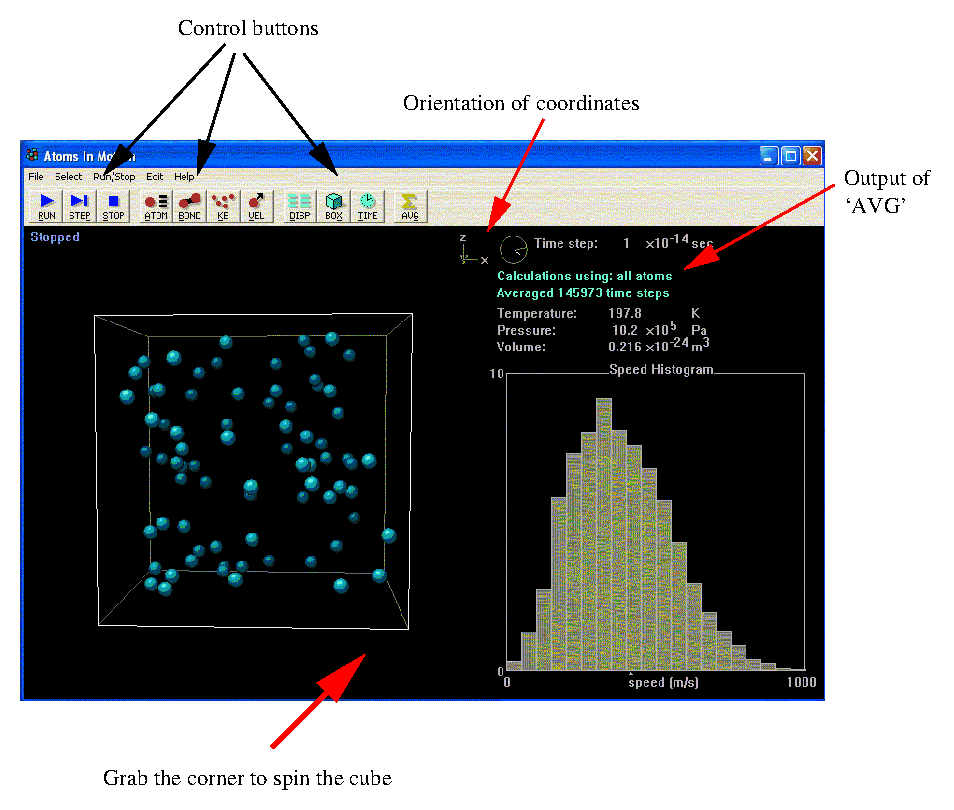
\includegraphics{am4a.eps}
\caption{{\it Atoms in Motion} window.}
\end{center}
\end{figure}

Can we use the concept of molecules behaving like little billiard
balls to explain why the ideal gas law relationship might hold? In
the next activity you are to pretend you are looking under a giant
microscope at a single spherical molecule as it bounces around in
a three-dimensional box by means of elastic collisions and that you
can time its motion and measure the distances it moves as a function
of time. 

If the molecule obeys Newton's Laws, you can calculate how the average
pressure that the molecule exerts on the walls of its container is
related to the volume of the box. The questions we have to consider
are the following. What is the momentum change as the
molecule bounces off a wall? How does this relate to the change in
the velocity component perpendicular to the wall? How often will our
molecule \char`\"{}hit the wall\char`\"{} as a function of its component
of velocity perpendicular to the wall and the distance between opposite
walls? What happens when the molecule is more energetic and moves
even faster? Will the results of your calculations based on mechanics
be compatible with the ideal gas law?

\textbf{Activity 2: The Theory of Atomic Motion}

(a) Stop the simulation if it's running and set the number of molecules to 
one. Do this by clicking on the {\it ATOM} button and getting a dialog box.
Enter `1' for the
number of Type A atoms and zero for all the others. Record the mass of the
Type A atom. Click {\it OK} and
the cube should now contain a single atom. If not, consult your instructor.
\vspace{20mm}

(b) The orientation of coordinates can be seen just above the right-hand corner
of the cube (consult Figure 1 also).
Suppose the molecule moves a distance 2$l$ (across the cube and back) in the $x$-direction in
a time \( \Delta t_{x} \). What is the equation needed to calculate
its $x$-component of velocity in terms of $l$ and \( \Delta t_{x} \)?
\vspace{20mm}

(c) Suppose the molecule moves a distance 2$l$ in the $y$-direction in
a time \( \Delta t_{y} \). What is the equation needed to calculate
its $y$-component of velocity in terms of $l$ and \( \Delta t_{y} \)?
\vspace{20mm}

(d) Suppose the molecule moves a distance 2$l$ in the $z$-direction in
a time \( \Delta t_{z} \). What is the equation needed to calculate
its $z$-component of velocity in terms of $l$ and \( \Delta t_{z} \)?
\vspace{20mm}

(e) We will now measure the average time $\Delta t_y$ for one complete round trip
from the left side of the cube to the right side and back again.
Click {\it AVG} and you will see some information printed in the color blue
on the right-hand side of the {\it Atoms-in-Motion} window (see also Figure 1).
The simulation takes small steps in time and calculates the positions of the
atoms at the end of each time step.
The number of these time steps taken is shown on the right-hand side and the size 
of each time step is printed at the top, right-hand-side of the window.
Using the {\it Step} button let the atom in the cube move until it bounces off the left wall of the cube. Stop the motion and record the number of the time step in the space below.
\vspace{20mm}

(f) Now run or step the simulation until the atom bounces across the cube, hits the right-hand wall, comes back and strikes the left hand wall again. Stop the motion and record the number of the time step.
Calculate $\Delta t_y$ and record it below.
\vspace{20mm}

(g) Each side of the cube has a length $l$ = $50 \times 10^{-10}$~m.
Combine this with the previous result to determine $v_y$ and record it.
\vspace{20mm}

(h) Repeat the above procedure for the top and bottom walls of the cube to get $v_z$.
\vspace{20mm}

(i) Rotate the cube by clicking and dragging one of the corners of the cube.
Spin it until you can see the atom bounces between the walls in the direction of
the $x$ coordinate.
Measure the $x$ component of the speed of the atom using the same procedure as before.
\vspace{20mm}

(j) Write the
expression for \( v_{total} \) in terms of the $x$, $y$, and $z$ components
of velocity. (Hint: This is an application of the 3-dimensional Pythagorean
theorem.) Determine $v_{total}$ for your atom.
We will use these results in a little while to calculate the pressure exerted by
our one-atom `gas'.
\vspace{20mm}

(k) Record the value of the pressure and temperature for your `gas' (as printed on the screen).
\vspace{20mm}

(l) If the collisions with the wall perpendicular to the $x$ direction
are elastic, show that the force exerted on that wall for each collision
is just \( F_{x}=2m\frac{v_{x}}{\Delta t_{x}} \)where m is the mass
of the particles and \( \Delta t_{x} \) the mean interval between
collisions with the wall. (Hint: Think of the form of Newton's second
law in which force is defined in terms of the change in momentum per
unit time so that \( F=\frac{\Delta p}{\Delta t} \).) \textbf{Warning:} Physicists too often use the same symbol to stand
for more than one quantity. In this case, note that \( \Delta p \)
(where {}``p'' is in lower case) indicates the change in \emph{momentum},
not pressure.
\vspace{20mm}

(m) Substitute the expression from part (b) for \( \Delta t_{x} \)
to show that 

\[
F_{x}=\frac{mv_{x}^{2}}{l}\]

\vspace{20mm}

(n) We have assumed from the beginning that we have a cubical box of edge length $l$. Show that the pressure on the wall perpendicular to the x axis caused by
the force \( F_{x} \) due to \emph{one} molecule is described by
the following expression.

\[
P=\frac{mv_{x}^{2}}{l^{3}}\].

\vspace{5mm}

(o) Now if we write the volume of our box as \( V=l^{3} \), the pressure becomes

\[
P=\frac{mv_{x}^{2}}{V}\].

(p) Now suppose that there are not one but N molecules in the box. What
is the pressure on the wall now?
\vspace{20mm}

(q) You have seen earlier that the three components of velocity for your single molecule were all different.  But averaged over $many$ molecules, the three components will have equal speeds.  In other words, \( \overline{v_{x}^{2}}=\overline{v_{y}^{2}}=\overline{v_{z}^{2}} \) where the bars indicate averages. If this is the case, then use the result of part (j) to show that

\[
\overline{v_{x}^{2}}=\frac{\overline{v_{total}^{2}}}{3}\].


(r) Now show that 

\[
P=N\frac{m\overline{v_{total}^{2}}}{3V}\].

\vspace{20mm}

(s) Finally, since the average kinetic energy of a molecule is just

\[
<E_{kin}>=\frac{1}{2}m\overline{v_{total}^{2}}\]


show that the pressure in the box can be written in the following
way.

\[
P=\frac{2N<E_{kin}>}{3V}\]
\vspace{20mm}

(t) Use the previous result to calculate the pressure using $v_{total}$, the mass of the atom, $N$ and $V$ for your one-atom gas. Compare your result with the pressure you recorded above from the output of the simulation (part (k) above).
Do they agree? How would you account for any difference?
\vspace{20mm}
